\documentclass[11pt,letterpaper]{article}
\usepackage[utf8]{inputenc}

\usepackage{graphicx}
\usepackage{float}
\usepackage{titlepic}
\usepackage{wrapfig}
\restylefloat{figure}
\usepackage{caption}
\usepackage{import}
\usepackage[section]{placeins}
\usepackage{tikz}
\usepackage{tkz-berge}
\usetikzlibrary{positioning}
\usetikzlibrary{fit}
\usetikzlibrary{knots}
\usetikzlibrary{shapes.geometric}
\tikzset{LabelStyle/.style= {fill=white}}
\tikzset{VertexStyle/.append style={minimum size=24pt}}

\usepackage[colorinlistoftodos]{todonotes}
\usepackage{amsmath, amsthm, amsfonts, mathrsfs}
\usepackage{mathtools}
\usepackage{interval}
\usepackage{geometry}
\usepackage[hidelinks]{hyperref}

\usepackage{multicol}

\usepackage{ftnxtra}
\usepackage[notes,backend=biber]{biblatex-chicago}
\bibliography{essay-2}

\usepackage{setspace}

\theoremstyle{definition}
\newtheorem{defn}{Definition}[section]

\newenvironment{dedication}
  {\clearpage% we want a new page
   \thispagestyle{empty}% no header and footer
   \vspace*{\stretch{1}}% some space at the top
   \itshape% the text is in italics
   \raggedleft}
  {\par % end the paragraph
   \vspace{\stretch{3}} % space at bottom is three times that at the top
   \clearpage           % finish off the page
  }

\title{A Graph Theoretic Approach to Understanding}
\author{Bernardo Meurer}
\titlepic{\vfill\centering\import{./}{cover}\vfill}
\date{March 14, 2018}

\begin{document}
\maketitle
\newpage

\begin{dedication}
    In memory of Stephen Hawking, who passed away this morning.

    \vspace{20pt}
    It would not be much of a universe if it wasn't home to the people you love.

    --- Stephen Hawking
\end{dedication}
\tableofcontents
\newpage
\doublespacing%
\begin{abstract}
    This paper presents a proof from first principles of the equivalence between the process of significance, as defined by Lacan, and the Traveling Salesman Problem, as defined in Graph Theory. Showing the NP-Completeness of the Significance Problem, the paper describes an argument for the root of misinterpretations in Human communications.
\end{abstract}
\section{Introduction}
In order to understand the main discussion, basic concepts of a variety of seemingly disparate topics are required. In this section these topics are presented in a superficial and non-rigorous form, and references are given for more in-depth readings.

\subsection{Turing Machines}
Turing machines, first described by Alan Turing\autocite{turing_1937}, are simple abstract computational devices intended to help investigate the extent and limitations of what can be computed.\autocite{sep-turing-machine} A Turing machine \(T\) is a particular form of state machine, we shall carefully construct its mathematical structure by means of modeling a deterministic, one-tape Turing machine. As is well known,however, all models of deterministic Turing machines are equivalent.\autocite{kleene_1943}\autocite{post_1943}\autocite{post_1944}

\begin{defn}\label{def:turingm}
    A deterministic one-tape Turing Machine is specified by a finite set of states \(Q \), a finite input alphabet \(\Sigma \), a finite tape alphabet \(\Gamma \supset \Sigma \), and a \emph{transition function} \(\delta\colon Q\times\Gamma\to Q\times \Gamma\times \{L, R\} \), where \(L \) and \(R \) stand for left and right, respectively. We also assume that \(\Sigma \), \(\Gamma \), \( \{L, R\} \) are disjoint sets.\autocite{kleinberg_2012}\autocite{kleinberg_2013}

    Formally, a Turing machine \(T \) is a 9-tuple\autocite{kozen_1997}
    \[
        T = (Q, \Sigma, \Gamma, \triangleright,\sqcup,\delta,s,t,f)
    \]
    with
    \begin{itemize}
        \item \(Q \) is a finite set of states;
        \item \(\Sigma \) is a finite set comprising the input alphabet;
        \item \(\Gamma \) is a finite set, comprising the tape alphabet, and containing \(\Sigma \);
        \item \(\sqcup \), \(\triangleright \) are the blank symbol, and the left end-marker respectively., with \( \{\sqcup, \triangleright \}\subset\Gamma \setminus \Sigma \);
        \item The transition function \(\delta\colon Q\times\Gamma\to Q\times \Gamma\times \{L, R\} \);
        \item \( \{s,t,f\}\subset Q \), the start, true (accept), and false (reject) states, respectively, with \(t \neq f \);
    \end{itemize}
\end{defn}

With this, the behavior of \(\delta \) is trivially understandable, and can be verbalized. To say \(\delta(\alpha, \beta) = (\phi,\kappa,\upsilon) \) is to say ``When in the state \(\alpha \), looking at the symbol \(\beta \), write the symbol \(\kappa \), move in the direction \(\upsilon \), and change to state \(\phi \).''\autocite{sep-turing-machine}

\subsection{Computability}
\begin{defn}\label{def:config}
    With \(\Sigma^* \) being the set of all finite sequences of elements of \(\Sigma \), and for \(x\in\Sigma^* \), \(x_0,\ldots,x_{n-1} \) denoting the elements of the sequence \(x \), where \(n \) is the \emph{length} of \(x \), denoted \(|x| \).

    A \emph{configuration} of a Turing Machine is an ordered triple \((\beta, \alpha, k)\in\Sigma^*\times Q\times \mathbb N \), where \(\beta \) is the string on the tape, \(\alpha \) is the machine's current state, and \(k \) denotes the position of the machine on the tape. \(\beta \) must begin with \(\triangleright \) and end with \(\sqcup \), and \(k \) must satisfy \(0\leq k \leq |\beta| \).\autocite{kleinberg_2012}
\end{defn}

The \emph{computation} of a Turing machine \(M \) is a sequence of configurations \(\beta_i, \alpha_i, k_i \), where \(i \) runs from \(0 \) to \(T \), satisfying:
\begin{itemize}
    \item \(M \) starts in a valid starting configuration, meaning that \(\alpha_0 = s \) and \(k_0 = 0 \);
    \item Each pair of configurations represents a valid transition.

        \(\forall i\in\interval[open right]{0}{T}\qquad(\beta_i, \alpha_i, k_i)\xrightarrow{M}(\beta_{i+1}, \alpha_{i+1}, k_{i+1}) \)

    \item if \(T = \infty \), we state that the computation \emph{does not halt.}
    \item if \(T < \infty \), we require that \(\alpha_T \in \{t, f\} \), and we say the computation \emph{halts}.
\end{itemize}

If we are able to construct \(M\) such that it solves a certain problem \(P\), which is to say that \(M\) halts, we say that \(P\) is computable. When we discuss the time-complexity of \(P\)\footnote{When referring to the complexity of a problem \(P\), it is implicit that a particular algorithm that solves \(P\), usually the most efficient, is meant.}, we discuss the \(T\) required so that said \(M\) halts.

With Definitions~\ref{def:config} and~\ref{def:turingm}, the reader now has a clear, formal, understanding of what a Turing machine is, and of what it means to be computable. This definitions will be used implicitly here on after.

\subsection{Complexity Theory}
Computational complexity theory is a sub-field of theoretical computer science whose primary goal is to classify and compare the practical difficulty of solving problems about finite objects.\autocite{sep-computational-complexity} Complexity Theory, therefore, aims in part to create meaningful taxonomies for the wide variety of problems that are determined as being computable. Here we use the term computable to mean that there exists a configuration for a Turing Machine which, given a finite amount of time, will solve the problem, and subsequently halt.

\subsection{Complexity Classes}

\begin{wrapfigure}{r}{0pt}
    \centering
    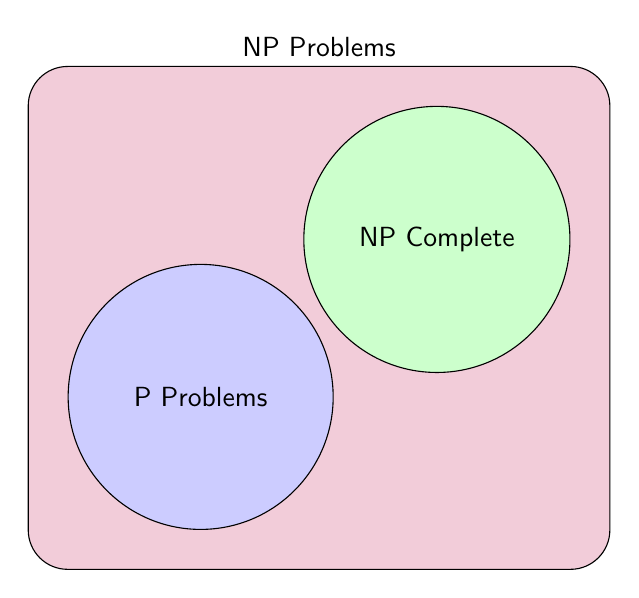
\begin{tikzpicture}[font=\sf]
        \pgfdeclarelayer{background}
        \pgfsetlayers{background,main}
        \tikzset{set/.style={draw,circle,inner ysep=10pt,align=center}}
        \node[set,fill=blue!20,text width=3cm](P) at (0, -1) {P Problems};
        \node[set,fill=green!20,text width=3cm](NP) at (3,+1) {NP Complete};
        \begin{pgfonlayer}{background}
            \node[fill=purple!20, fit=(P)(NP),draw,rounded corners=0.5cm,inner sep=.5cm,label={NP Problems}]{};
        \end{pgfonlayer}
    \end{tikzpicture}
    \caption{NP Complexity Class}
\end{wrapfigure}
There is a large number of complexity classes that problems can belong to. Firstly, a distinction must be made between time-complexity and space complexity. While space-complexity refers to the amount of memory, cells in our model of \(M\), needed for \(M\) to compute a certain \(P\), time-complexity refers to the number of state-transitions \(M\) performs until halting. Note that both space and time complexity will usually be presented in a form dependent on the number of elements involved in the particular instance of the problem.

Of particular interest, are problems with Non-deterministic Polynomial Time complexity (NP), and it's subset classes P, and NP-Complete. For a problem to belong in NP, a deterministic Turing machine must be able to \emph{verify} that a solution for it is valid in polynomial time. P-type problems are also \emph{solved} in polynomial time, and it follows from Cobham-Edmonds thesis that they are usually tractable\autocite{cobham_1965}, although this does not always hold\autocite{goldreich_2008}. Here, \emph{tractable} refers to the \emph{feasibility} of the problem. A problem might be solvable given an absurdly, albeit finite, amount of resources (time and space), but in reality that solution is not feasible, in which case we call that problem \emph{intractable}. NP-Complete problems, on the other hand, are intractable, and although verifying a solution is simple (for they are in NP,) finding a solution is not. Moreover, it is characteristic of NP-Complete problems that as the size of the problem grows, the time required to solve them grows extremely fast.\autocite{sep-computational-complexity} Formally,

\begin{defn}
    A decision problem \(D\) is NP-Complete iff:
    \begin{enumerate}
        \item \(D\in\text{NP}\)
        \item \((\forall P\in\text{NP})(P\leq_m^P D)\), where \(\leq_m^P\) denotes a Karp reduction\autocite{karp_1972}.\autocite{cook_1971}
    \end{enumerate}
\end{defn}

\begin{defn}
    A decision problem \(D\) is in P, or PSPACE iff there exists a deterministic Turing machine \(M\) such that \(M\) runs in polynomial time.\autocite{leeuwen_1994}
\end{defn}
\newpage
\subsubsection{Examples}
\begin{multicols}{2}
    Problems in PSPACE
    \begin{itemize}
            \item Finding Greatest Common Divisors;
            \item Defining the Independent Edge Set of a graph;
            \item Determining primality
    \end{itemize}
    \columnbreak
    NP-Complete Problems
    \begin{itemize}
        \item Boolean Satisfiability (SAT)
        \item Hamiltonian Path Problems
        \item Traveling Salesman Problem (TSP)
        \item Graph Coloring Problem
        \item Vertex Covering Problem
    \end{itemize}
\end{multicols}


\subsection{Graphs}
\begin{wrapfigure}{l}{0pt}
    \centering
    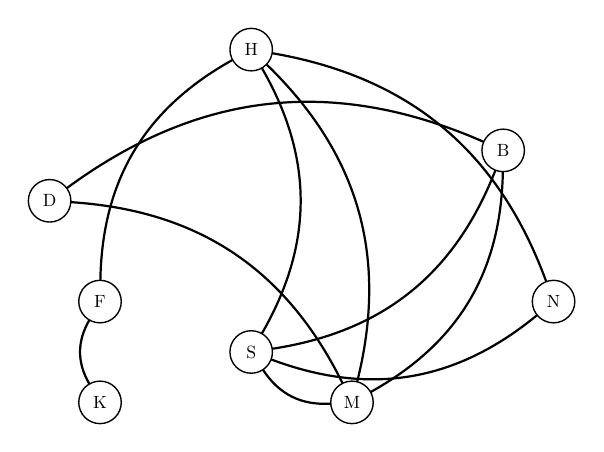
\begin{tikzpicture}[scale=0.64,transform shape]
        \Vertex[x=0,y=0]{K}
        \Vertex[x=0,y=2]{F}
        \Vertex[x=-1,y=4]{D}
        \Vertex[x=3,y=7]{H}
        \Vertex[x=8,y=5]{B}
        \Vertex[x=9,y=2]{N}
        \Vertex[x=5,y=0]{M}
        \Vertex[x=3,y=1]{S}
        \tikzstyle{LabelStyle}=[fill=white,sloped]
        \tikzstyle{EdgeStyle}=[bend left]
        \Edges(K,F)
        \Edges(H,S)
        \Edges(H,M)
        \Edges(D,B)
        \Edges(D,M)
        \Edges(B,M)
        \Edges(H,N)
        \Edges(F,H)
        \tikzstyle{EdgeStyle}=[bend right]
        \Edges(S,B)
        \Edges(S,N)
        \Edges(S,M)
    \end{tikzpicture}
    \caption{A Graph}\label{fig:graph}
\end{wrapfigure}
A variety of real-world problems can easily be described by using a diagram consisting of a set of points, with lines joining certain pairs of these points.\autocite{bondy_murty_2008} These diagrams we call \emph{Graphs}, and formally we define them as follows
\begin{defn}\label{def:graph}
    A \emph{graph} \(G\) is an ordered pair \((V(G), E(G))\) consisting of a set \(V(G)\) of \emph{vertices} and a set \(E(G)\), disjoint from \(V(G)\), of \emph{edges}, together with an \emph{incidence function} \(\psi_G\) that associates with each edge of \(G\) an unordered pair of (not necessarily distinct) vertices of \(G\). If \(\epsilon \) is an edge, and \(u\), \(v\) are vertices such that \(\psi_G(\epsilon)=\{u,v\} \), then \(e\) is said to \emph{join} \(u\) and \(v\), and the vertices \(u\) and \(v\) are called the \emph{ends} of \(e\).\autocite{bondy_murty_2008}
\end{defn}

\subsection{The Traveling Salesman Problem}\label{sub:tsp}
\begin{wrapfigure}{r}{0pt}
    \centering
    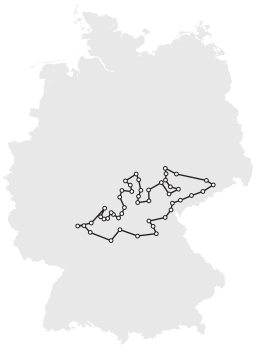
\includegraphics{./TSP.png}
    \caption{A traveling salesman tour.\protect\footnotemark[21]}\label{fig:TSP}
\end{wrapfigure}
Given a set of cities along with the cost of travel between each pair of them, the Traveling Salesman Problem (TSP) is to find the cheapest way of visiting all the cities and returning to the starting point. The ``way of visiting all the cities'' is simply the order in which the cities are visited; the ordering is called a tour or circuit through the cities.\autocite{applegate_2007}

If one looks at Figure~\ref{fig:TSP} through the optics of Definition~\ref{def:graph} it becomes clear that the cities the salesman must go through can be modeled as vertices in a graph. We can then formally define the TSP as

\begin{defn}[TSP]\label{def:TSP}
    Let \(V\) be a set of vertices, \(f\colon V\times V \to \mathbb Z\) some function, and \(t\in \mathbb Z\). The Traveling Salesman Problem (TSP) is finding \((G, f, t)\) such that \(G\) is a complete graph, and its tour cost does not exceed \(t\).
\end{defn}

Therefore, for any graph \(G\), it's possible for us to describe the TSP over it, and indeed, given enough time, compute it. Note that the problem of ``Finding the shortest path along \(G\) that passes through the proper subset \(S\subset G\)'' is reducible, and therefore equivalent, to the TSP, for it is nothing more than the TSP on a subset of \(G\).

\subsection{Borromean Knots}
\begin{wrapfigure}{r}{0pt}
    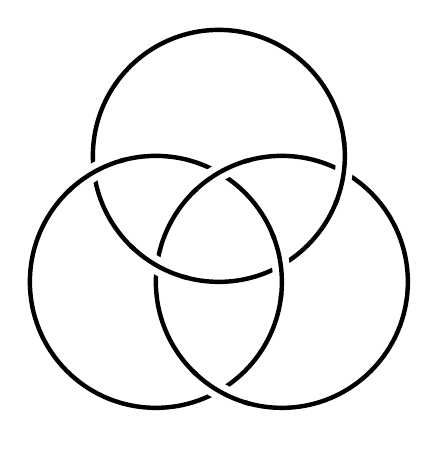
\begin{tikzpicture}[scale=1.6]
        \begin{knot}[clip width=4]
            \strand [ultra thick] (0,0) circle (1.0cm);
            \strand [ultra thick] (1,0) circle (1.0cm);
            \strand [ultra thick] (0.5,1) circle (1.0cm);
            \flipcrossings{1, 2, 5, 6}
        \end{knot}
    \end{tikzpicture}
    \caption{Borromean Knot}\label{fig:borromean}
\end{wrapfigure}
In his meditations on the topology of Borromean knots, and in particular throughout his seminar of 1974--1975, the French psychoanalyst Jacques Lacan exposes the interrelation between the Symbolic, the Imaginary, and the Real in terms of link-topology\autocite{rolfsen_2004}\footnote{Although Lacan, and the Stanford Encyclopedia, speak of \emph{knot-topology}, that is mathematically unsound. The Borromean Knot is a Link, and not a Knot as one would presume from its name.}. Lacan calls each of these ``rings'' of the knot a \emph{register}.

\begin{defn}\label{def:imaginary}
    The Imaginary is generally associated with the restricted spheres of consciousness and self-awareness. Who and what one ``imagines'' other persons to be, what one thereby ``imagines'' they mean when communicatively interacting, who and what one ``imagines'' oneself to be, including from the imagined perspectives of others—all of the preceding is encompassed under the heading of this register. The Imaginary is an intrinsic, unavoidable dimension of the existences of speaking psychical subjects, it is the field of the ego.\autocite{sep-lacan}
\end{defn}
\begin{defn}\label{def:symbolic}
    The Symbolic refers to the customs, institutions, laws, mores, norms, practices, rituals, rules, traditions, and so on of cultures and societies (with these things being entwined in various ways with language).\autocite{sep-lacan}
\end{defn}
\begin{defn}\label{def:real}
    The Real is that which is neither symbolic nor imaginary. It is always mediated by the other two others of the Knot, since it can never be truly known.
\end{defn}

The usage of the Borromean topology here to link is crucial, and extremely meaningful. It is idiosyncratic of this topology that there is no hierarchical order between the rings, that none of the rings intersect, and that breaking \emph{any} of the three rings will immediately liberate the remaining. It is clear what implications these characteristics have to the proposed interaction of the Real, Symbolic, and Imaginary.

\subsection{The other and the Other}

Throughout his work, Lacan makes use of two grammatically similar albeit semantically disparate terms: other, and Other. Namely,
\begin{defn}\label{def:little-other}
    The other, sometimes referred to as little-other, is the ego (part of the Imaginary register) and its alter-egos. Therefore both the self, and others (as in other people) are included in the little-other.\autocite{sep-lacan}
\end{defn}
\begin{defn}\label{def:big-other}
    The Other, referred to as big-Other, is usually defined in terms of the Symbolic register, in which case it is the ``objective spirit'' of socio-linguistic structures in inter-subjective interactions, i.e.\ the Symbolic order itself.\autocite{sep-lacan}
\end{defn}

The philosopher Slavoj Žižek in his works relating to Ideology, will often argue that Ideology, as defined by himself, is closely related to the Other, in fact at times it is fair to say Ideology is part of the Other, as will be shown later.
\newpage
\subsection{The Signifier and the Signified}
\begin{wrapfigure}{r}{4cm}
    \centering
    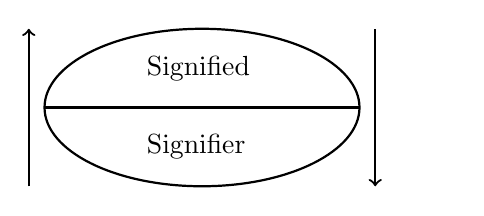
\begin{tikzpicture}
        \draw[thick,->] (0,-1) -- (0, 1);
        \draw[thick] (2.2,0) ellipse (2cm and 1cm);
        \draw[thick,<-] (4.4,-1) -- (4.4, 1);
        \draw[very thick] (.2,0) -- (4.2,0);
        \node[text width = 3.8cm] at (3.4,-.5){Signifier};
        \node[text width = 3.8cm] at (3.4,.5){Signified};
    \end{tikzpicture}
    \caption{The Signifier and the Signified}\label{fig:sig}
\end{wrapfigure}
In his famous book \textit{Course in General Linguistics}\autocite{saussure_bally_sechehaye_urbain_riedlinger_2016}, Ferdinand de Saussure provides us with a careful description for the workings of language, including the definitions of two of the main concepts of semiotics, the \emph{Signifier}, and the \emph{Signified}.

\begin{defn}\label{def:signifier}
    The \emph{Signifier} is the concrete object of language, be it a word, a gesture, or any other form of linguistics.\autocite{berger_2013}
\end{defn}
\begin{defn}\label{def:signified}
    The \emph{Signified} is the abstract object of language, which is to say a mental concept, i.e.\ that which a signifier signifies.\autocite{berger_2013}
\end{defn}
As an example of this, when one reads the word ``Volume,'' the very word is the signifier, and the idea of volume, the abstract, mental concept of it, is the signified.

While for Saussure the connection between the signifier and the signified (signification) is very strict and unbreakable, being an injective-type function described through Saussurean algorithm, Lacan has a very distinct view. For Lacan, the signifier is prior to the signifieds, which are solely produced by the combination of the signifiers. Signification, therefore, is not a stable relation, but a process where the signifiers produce the signified by the means of metaphor and metonymy.\autocite{lacan_miller_2000}

\newpage
\section{Graphs and Understanding}

Lacan shows us throughout his seminars that, as oppose to Saussure's classical work in Linguistics, language is not a system of signifieds (of meanings), but rather a system of signifiers, that themselves changeably produce the signified. In order to produce the signified individuals make use of contextual cues in their reality\footnote{Loosely defined here} to provide them with a reasonable resulting signified from their perspective.

Given a set of signifiers which form a sentence \(\mathfrak{s}\), there are a number of semi-signifieds one can produce, which themselves are combined into yet another layer of semi-signifieds, until we finally are able to produce the signified \(\mathscr{S}\). These intermediate representations, and most importantly the extreme quantity of them, are the central reason to the non-static nature of \(\mathscr{S}\).

\begin{minipage}{\linewidth}
    \makebox[\linewidth]{
        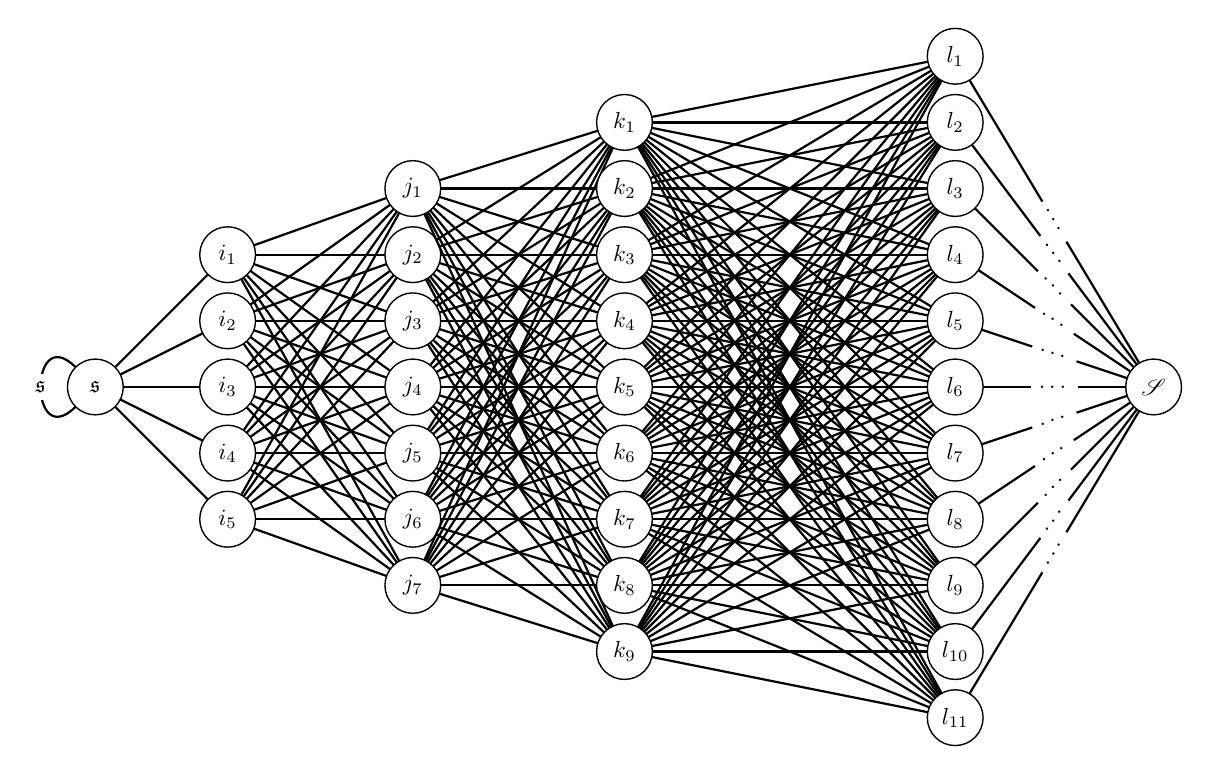
\begin{tikzpicture}[scale=0.84, every node/.style={scale=0.84}]
            \SetVertexMath
            \Vertex[x=-8, y=0,L=\mathfrak{s}]{s}
            \Loop[dist=1cm,label={$\mathfrak{s}$},style={thick,-}](s)
            \Vertex[x=8, y=0,L=\mathscr{S}]{S}

            \foreach \y [count=\n,evaluate={\m=int(6-\n)}] in {2,...,-2}
                {\Vertex[x=-6, y=\y, L=i_\n]{l1\m}
                    \Edges(s, l1\m)}

            \foreach \y [count=\n,evaluate={\m=int(8-\n)}] in {3,...,-3}
                {\Vertex[x=-3.2, y=\y, L=j_\n]{l2\m}
                    \foreach \k in {1,...,5}
                        {\Edges(l1\k, l2\m)}}

            \foreach \y [count=\n,evaluate={\m=int(10-\n)}] in {4,...,-4}
                {\Vertex[x=0, y=\y, L=k_\n]{l3\m}
                    \foreach \k in {1,...,7}
                        {\Edges(l2\k,l3\m)}}

            \foreach \y [count=\n,evaluate={\m=int(12-\n)}] in {5,...,-5}
            {\Vertex[x=5, y=\y, L=l_{\n}]{l4\m}
            \draw[-,thick] (l4\m)--(S) node[midway,sloped,fill=white]{$\dots$};
            \foreach \k in {1,...,9}
                {\Edges(l3\k,l4\m)}}
        \end{tikzpicture}}
    \captionof{figure}{Graph of paths from the set of signifiers \(\mathfrak{s}\) to the signified \(\mathscr{S}\).}\label{fig:lgraph}
\end{minipage}
\newpage
Figure~\ref{fig:lgraph} shows what the graph for the process of understanding a sentence \(\mathfrak{s}\) looks like, \(i_n, j_n, k_n, l_n\) are all intermediate states in the process of signification. Usually, when we speak of \emph{misunderstanding} a sentence, we speak of either interpreting one of the intermediate states as the final signifier \(\mathscr{S}\), or arriving at a completely different \(\mathscr{S}\) by means of using differing intermediates states from the originator.

Therefore, if we say that each edge on the graph of Figure~\ref{fig:lgraph} has a weight that is inversely proportional to the closeness of its path to the path taken by the originator in the formulation of \(\mathfrak{s}\), we can state that the process of correct signification, by which we mean arriving at the originator's signified through the same intermediate states, is Karp-reducible to the TSP, and is therefore NP-Complete.

To show this, we use the finishing note of Subsection~\ref{sub:tsp}. Since it is trivial, that the problem stated above is a case of finding the optimal path among a subset of the vertices of a Graph \(G\), we have that the problem is NP-Complete.
Note that, although the resulting graph isn't closed, as is required by the definition of the TSP (otherwise path-finding between two nodes is P-Complete via Dijkstra's algorithm) it is trivial to make it so, by requiring that the in the process of understanding one must also be able to reach \(\mathfrak{s}\) from \(\mathscr{S}\). In other words, by requiring that one must be able to form a sentence representing one's understanding.

The NP-Completeness of signification gives us an impressive result: Understanding sentences is an intractable problem. Given finite resources, which perhaps unfortunately is a boundary of the Human condition, there is no efficient way to compute for the answer of the Signification Problem. In other words, our deduction of the signified given a sentence is purely heuristic, and reliant on the aforementioned cues, for it is the only possible way to solve the problem in a timely manner. In those cues, the contextual setting one uses to interpret the signifiers in the process of signification, lies the entire reason for misunderstandings.

\section{Satire: A Case Study of Gulliver's Travels}
We see the world through Ideological Lens, that cause us to observe the world around us as being ``normal.'' In fact, Ideology itself is what causes us to define as normal that which we see daily and commonly. This idea, presented throughout Slavoj Žižek's work,\autocite{zizek_2012} is tightly knit with the concept of the Other, for Ideology becomes itself the symbolic order, which follows from a quasi-Wittgensteinian approach to the influence of the symbolic in the self. The Satirical has as its unifying feature the effort to subvert the Other, bypassing Ideology, in order to allow one to see oneself through the eyes of the other, the alter-ego of the self.

As an experiment, in order to show the subversion of the Other, imagine the first Man who, in his explorations, came across a strange, short, tree with uncommonly large, glossy leaves. On it grew, from some top branches that held a flower-like structure in its end, large groups of bow-shaped, cylinder-like, green and yellow semi-branches. The natives of this land seem to take only the semi-branches of a particular color, and open it to find a soft, white kernel which they eat. Although the description above might seem like that of an extraterrestrial encounter with a nature far differing from our own, with some good-faith one can see that, in fact, the banana tree is what's being described. The commonness of the banana makes it seem ordinary, but at first encounter and analysis it seems truly bizarre. There is no doubt that we are as bizarre to the unknown, as the unknown is to us. Žižek calls this filter and categorization of the normal Ideology, or the Ideological lens. For Žižek, Ideology and the Other are closely related, due to the Wittgensteinian notion of means as a message. Moreover, to speak of one's otherness is to speak of one perceiving the self as if it were a perception of someone else, i.e.\ to mistake the self for it's alter-ego, the other. This process breaks with the sense of normality that generally veils the analysis of that which is common, or known. Satire subverts the Other to allow the self to be seen through the eyes of the other, and thus weakening the Borromean knot by causing the Symbolic to disconnect with the Imaginary.

The method of description used above works because, as Lacan shows us, and in opposition to Saussure's traditional work, language is not a sign-system, but a system of signifiers. When  we engage in the description method, we carefully leave out contextual bits of information, the cues, that are paramount in the process of signification. Without the linking metadata attached to the signifiers, it becomes hard for the reader to correctly identify the signifieds, which is exactly how the subversion takes place. Ideology, the Other, operates on the level of the signifieds, not of the signifiers, and therefore this layer of confusion allows us to bypass it. One will happily read an essay on how the Yahoos battle in the mud for stones, but not about how petty the bullionist philosophy is. If we construct the former essay carefully, it can become hard for the reader to detect the true signified, at which point we've successfully subverted language, allowing us to bypass his ideological filters.

As we see in \textit{Body Ritual Among the Nacirema},\autocite{miner_1956} a veiled, yet accurate, description of ourselves can manage to bypass the ideological lens, at which point, and only by this means is this ever truly possible, we can look at ourselves and stand in awe of how bizarre we truly are. Even though Nacirema could be pointed out as not being a true satire, given that by most standards it isn't funny, it's impossible not to see the deeply satirical nature of it, and to draw some parallels with Jonathan Swift's \textit{Gulliver's Travels}. This same effect can be seen, for example, in the description of the Yahoos, and their addiction to colored stones,\autocite{swift_rivero_2002} a painful description of nothing if not ourselves, and in particular of the Bullionist theory that ruled the governing mindset in Swift's time. To bring it back to Lacanian terms, Satire allows us to lift the veil that is the Other (Symbolic Order) and, through a weakening of the Borromean ring, allow us to see the extraterraneousness of ourselves.

We live in an age where the value of self-correction has been, by and large, left aside. Social media, with the echo-chambers it provides, has fostered a culture where self-validation through repetition and isolation is the norm. This, perhaps, explains why Satire has changed so much in its form; we no longer see works like Swift's, or at least they don't rise to fame, because the fundamental dynamic that made it possible is gone. In \textit{Gulliver's Travels}, we see Swift's critiques of the English, and yet his reader is the Englishman himself. This is possible due to the ``veiled critique'' characteristic of his work, by which when the reader realizes he is being critiqued, it is far too late for he has already read and pondered on the work. Now, this has become impossible, partially because the isolation aspect makes critical works, however veiled, difficult to reach their intended audience, but also because work that requires reading and pondering in extension has grown out of fashion. The ``instant delivery'' aspect of modern culture makes it unlikely that any meaningful number of people would go through the trouble of reading something that is longer than a couple of pages, which makes it increasingly harder to construct a through, veiled, and entertaining critique like Swift's work. Interestingly this has caused the satiric dynamic to change dramatically: now each respective side of an issue consumes the satire that was meant for their opponents, since they can and want to see the critique contained in it, as it feeds into their belief-loop. Because of this we have seen the slow disappearing of the veil, transforming satire into mere parody, as is clear from any number of late night shows, who would be categorized as satire, even if they are just comedic-political autofellatio.

Satire, given its kernel-factor as presented here, requires from the reader some a priori knowledge, namely, it requires broad contextual awareness to correctly signify it, but must importantly it takes interest in the other. Satire, once more, describes the self of the one being criticized as if it were the (little) other, and therefore it requires the reader to have some interest in the other, since that not being present would making reading the satire pointless at first (given the delayed realization of the true meaning of the work.) Herein lies the cause for the slow, but steady, disappearance of satire: there is no longer any interest in the other. The central assumption that allows for the satirical delivery, and opens the reader to the material, is by and large gone, and so is true satire.

\newpage
\printbibliography[heading=bibintoc,title={Bibliography}]
\end{document}
